\documentclass[a4paper,12pt]{article}
\usepackage[utf8]{inputenc}
\usepackage{pgfplots}
\usepackage[hidelinks]{hyperref}
\usepackage[left=2cm,top=2cm,right=2cm,bottom=2cm]{geometry}

%opening
\title{Autonomous Agents - Assignment 3 Report}
\author{Nicolò Girardi, Jorge Sáez Gómez, Johan Sundin}

\begin{document}

\maketitle

\section{Introduction}
In this assignment we worked on a predator versus prey grid world scenario, in which both the predator and the prey are learning agents  \cite{Assignment}. \cite{vlasis} There are small changes made to the grid world scenario compared to previous assignments.%We have implemented and evaluated several algorithms for each agent to use. For one algorithm, Independent Q-Learning, we have used a scenario in which several predators chase a single prey. The results of these evaluations will be presented in section 3.

\section{Theoretical description of the algorithms}
For this assignment we have implemented the following algorithms: Independent Q-Learning \cite{vlasis}, Minimax Q-Learning \cite{minimax}, Generalized Infinitesimal Gradient Ascent Win or Learn Fast(GIGA-WoLF) \cite{GIGA-wolf}. Each algorithm will be described concisely below.

\subsection{Independent Q-Learning}
In Independent Q-Learning each agent in the environment treats all other agents as being part of the environment. An agent employing Independent Q-Learning does not try to model other agents, or try to learn their behavior \cite{vlasis}. The agent then uses Q-Learning to learn a state-actionvalue function, mapping actions in states to values.
A problem with this algorithm is that the Q-Learning algorithm assumes a static environment, in which state transition probabilities do not change. This assumption is not valid for independent Q-Learning, as other learning agents might change their behavior over time. Since the agent models other agents as part of the environment, the environment thus becomes dynamic.
\subsection{Minimax Q-Learning}
\subsection{GIGA-WoLF}

\section{Method}

Something here...

\subsection{Scoring system}

$$ score = reward \cdot 0.9^{T - 1} $$

\subsection{State-space encoding}

In order to make the presented algorithms converge as fast as possible, we made use of the reduced state-space we devised for the first assignment. However, we had to adapt it to the multi-predator scenario in order to make it work with all cases we will be considering for this assignment. To this end, several ideas needed to be introduced.

First of all, we will extend our original idea for a reduced state-space encoding and use the distances from a certain agant to the rest of them, instead of encoding the positions of every agent on the world. This allows us to use two less variables for the state-space encoding. Furthermore, it is now essential to know which agent ``we are'', and this needs to be encoded in the state representation somehow. If this information was not encoded, then it would be impossible to distinguish between predators in a multi-predator setting, and the algorithms would not be able to know which predator should be applied a certain action from the usual set \{North, South, East, West, Stay\}.

\section{Results}

Something here...

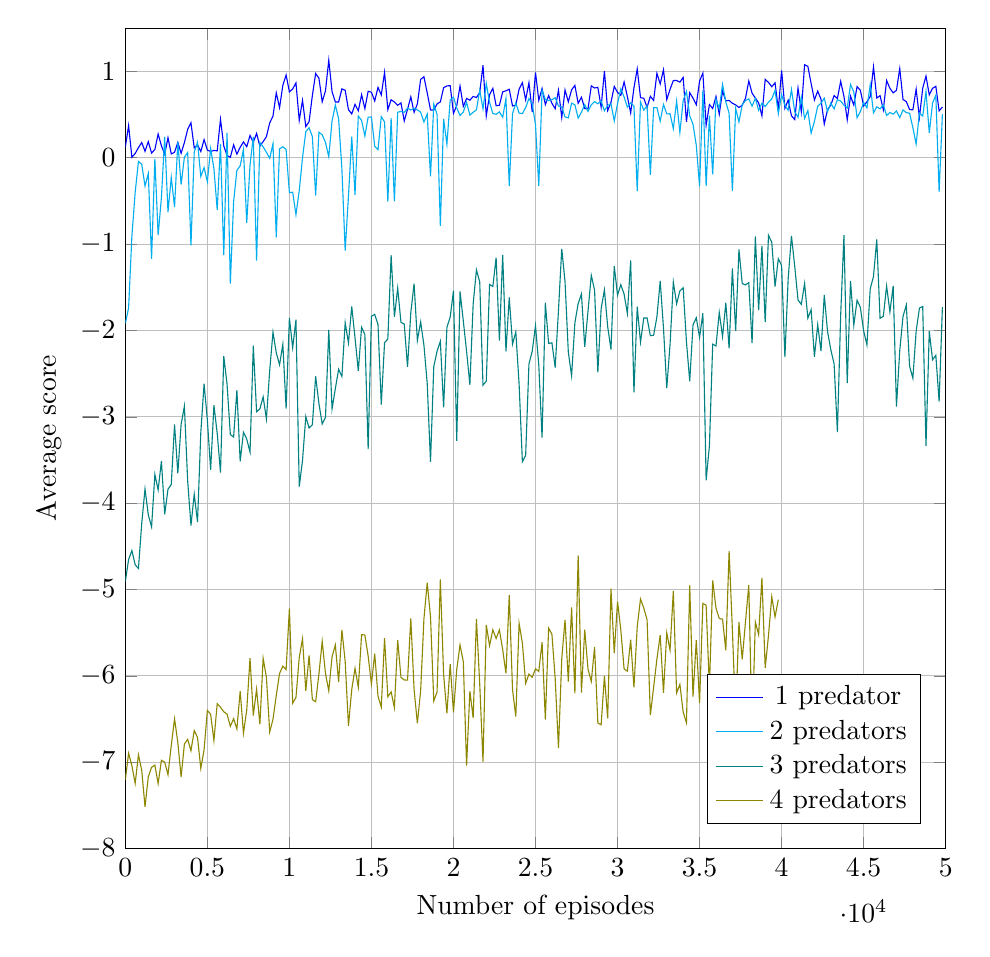
\begin{tikzpicture}
\begin{axis}[height=12cm, width=12cm, grid=major, xlabel=Number of episodes, ylabel=Average score, xmin=0, xmax=50000, ymin=-8, ymax=1.5, legend pos=south east]
\addplot[blue] coordinates {
(0, 0.12311333) (200, 0.37291035) (400, 0.005859607) (600, 0.049466293) (800, 0.11737791) (1000, 0.17613216) (1200, 0.07521633) (1400, 0.18682627) (1600, 0.05445082) (1800, 0.09551313) (2000, 0.27491662) (2200, 0.13851231) (2400, 0.040507913) (2600, 0.23153378) (2800, 0.043900598) (3000, 0.06416984) (3200, 0.17793338) (3400, 0.05202268) (3600, 0.17570023) (3800, 0.32845342) (4000, 0.40452927) (4200, 0.11411854) (4400, 0.14853871) (4600, 0.07157968) (4800, 0.21031915) (5000, 0.08820571) (5200, 0.072937086) (5400, 0.08486481) (5600, 0.07941788) (5800, 0.4452494) (6000, 0.13701701) (6200, 0.025847754) (6400, 0.004841691) (6600, 0.14917505) (6800, 0.04229796) (7000, 0.121590786) (7200, 0.18316235) (7400, 0.12732571) (7600, 0.25809836) (7800, 0.17852926) (8000, 0.28181237) (8200, 0.13457195) (8400, 0.18755656) (8600, 0.24483277) (8800, 0.4035685) (9000, 0.48188838) (9200, 0.7513958) (9400, 0.5798128) (9600, 0.83779556) (9800, 0.9586124) (10000, 0.76200897) (10200, 0.7967857) (10400, 0.86692333) (10600, 0.4330651) (10800, 0.6652868) (11000, 0.3608077) (11200, 0.41720352) (11400, 0.7206782) (11600, 0.9752733) (11800, 0.92140144) (12000, 0.64785194) (12200, 0.7753569) (12400, 1.1302389) (12600, 0.76504636) (12800, 0.6460804) (13000, 0.6453099) (13200, 0.79733175) (13400, 0.7816915) (13600, 0.5568686) (13800, 0.50720525) (14000, 0.6182007) (14200, 0.54308236) (14400, 0.72989583) (14600, 0.5691778) (14800, 0.76986367) (15000, 0.75844496) (15200, 0.6575198) (15400, 0.814738) (15600, 0.72703487) (15800, 0.98957306) (16000, 0.55759645) (16200, 0.67091566) (16400, 0.64596766) (16600, 0.60687184) (16800, 0.63569313) (17000, 0.42546326) (17200, 0.56136364) (17400, 0.70533943) (17600, 0.526573) (17800, 0.62348706) (18000, 0.90752506) (18200, 0.93750405) (18400, 0.7518081) (18600, 0.55356145) (18800, 0.5527333) (19000, 0.6229305) (19200, 0.64682955) (19400, 0.81080806) (19600, 0.83201253) (19800, 0.8350899) (20000, 0.51495993) (20200, 0.60367537) (20400, 0.83035755) (20600, 0.594895) (20800, 0.68623) (21000, 0.6662826) (21200, 0.71033686) (21400, 0.696892) (21600, 0.7549724) (21800, 1.0706741) (22000, 0.48375833) (22200, 0.73100114) (22400, 0.80411315) (22600, 0.60265803) (22800, 0.60719985) (23000, 0.7628744) (23200, 0.7751014) (23400, 0.79276013) (23600, 0.5995053) (23800, 0.60920525) (24000, 0.79524785) (24200, 0.8686073) (24400, 0.67053753) (24600, 0.86897624) (24800, 0.530098) (25000, 0.98808223) (25200, 0.66511005) (25400, 0.80210364) (25600, 0.61496335) (25800, 0.7197734) (26000, 0.6306582) (26200, 0.5673961) (26400, 0.7825887) (26600, 0.46658596) (26800, 0.78488076) (27000, 0.64838743) (27200, 0.7862601) (27400, 0.83730656) (27600, 0.6311794) (27800, 0.70044917) (28000, 0.56972855) (28200, 0.5652089) (28400, 0.83283055) (28600, 0.80763096) (28800, 0.8154031) (29000, 0.58667314) (29200, 1.0039911) (29400, 0.54685885) (29600, 0.64115965) (29800, 0.82638836) (30000, 0.7565814) (30200, 0.72281563) (30400, 0.8781006) (30600, 0.7074866) (30800, 0.51842356) (31000, 0.8090357) (31200, 1.0285946) (31400, 0.6957286) (31600, 0.6890055) (31800, 0.5831901) (32000, 0.71191686) (32200, 0.66293126) (32400, 0.97838193) (32600, 0.85442805) (32800, 1.0186008) (33000, 0.6731355) (33200, 0.7920691) (33400, 0.89382666) (33600, 0.89441955) (33800, 0.875887) (34000, 0.9308016) (34200, 0.41515762) (34400, 0.7541516) (34600, 0.68967533) (34800, 0.6128123) (35000, 0.88829285) (35200, 0.9801734) (35400, 0.37671837) (35600, 0.6159856) (35800, 0.56980926) (36000, 0.7098284) (36200, 0.5036374) (36400, 0.77363306) (36600, 0.65814906) (36800, 0.6641292) (37000, 0.6302255) (37200, 0.6118248) (37400, 0.5816266) (37600, 0.60756665) (37800, 0.6900208) (38000, 0.8891732) (38200, 0.7472557) (38400, 0.6912061) (38600, 0.6355242) (38800, 0.48562765) (39000, 0.9072425) (39200, 0.87221575) (39400, 0.82227844) (39600, 0.8674716) (39800, 0.55969286) (40000, 1.0123445) (40200, 0.5727665) (40400, 0.6666588) (40600, 0.48632938) (40800, 0.44210234) (41000, 0.8067209) (41200, 0.5338333) (41400, 1.0775373) (41600, 1.0583549) (41800, 0.8582168) (42000, 0.6688322) (42200, 0.7719201)
 (42400, 0.6783194) (42600, 0.39015734) (42800, 0.5586302) (43000, 0.60920686) (43200, 0.7198567) (43400, 0.68543106) (43600, 0.88556534) (43800, 0.71035475) (44000, 0.43958923) (44200, 0.71291566) (44400, 0.61034644) (44600, 0.8237655) (44800, 0.7812962) (45000, 0.600354) (45200, 0.64789253) (45400, 0.7088817) (45600, 1.0528073) (45800, 0.6915912) (46000, 0.7195931) (46200, 0.5560597) (46400, 0.89496577) (46600, 0.8038976) (46800, 0.75193614) (47000, 0.7810347) (47200, 1.0323086) (47400, 0.6744882) (47600, 0.65002835) (47800, 0.55864114) (48000, 0.5548241) (48200, 0.79452276) (48400, 0.46607953) (48600, 0.80551004) (48800, 0.9458439) (49000, 0.727809) (49200, 0.8037875) (49400, 0.82720166) (49600, 0.5427888) (49800, 0.5866451)
};
\addlegendentry{1 predator}

\addplot[cyan] coordinates {
(0, -1.9205298) (200, -1.7388507) (400, -0.9073605) (600, -0.40102953) (800, -0.042787094) (1000, -0.07577009) (1200, -0.32746255) (1400, -0.18341602) (1600, -1.170195) (1800, -0.013471894) (2000, -0.8964232) (2200, -0.461334) (2400, 0.24141155) (2600, -0.6283368) (2800, -0.2283712) (3000, -0.57258445) (3200, 0.17929102) (3400, -0.31166205) (3600, 0.007062384) (3800, 0.06026135) (4000, -1.0149127) (4200, 0.06476224) (4400, 0.18024637) (4600, -0.2161829) (4800, -0.11383107) (5000, -0.27707076) (5200, 0.10567677) (5400, -0.12654133) (5600, -0.6028171) (5800, 0.16143693) (6000, -1.1277615) (6200, 0.28646076) (6400, -1.4571576) (6600, -0.50730574) (6800, -0.14445731) (7000, -0.0942236) (7200, 0.09596811) (7400, -0.75506026) (7600, -0.0838999) (7800, 0.2416222) (8000, -1.1905707) (8200, 0.17853034) (8400, 0.12540622) (8600, 0.063145675) (8800, -0.0074097943) (9000, 0.16381152) (9200, -0.92104495) (9400, 0.103478506) (9600, 0.12659189) (9800, 0.09520874) (10000, -0.40493932) (10200, -0.3984471) (10400, -0.6590253) (10600, -0.38123265) (10800, 0.0012456184) (11000, 0.3017538) (11200, 0.34769523) (11400, 0.24596472) (11600, -0.43972054) (11800, 0.29495072) (12000, 0.26569435) (12200, 0.17736508) (12400, 0.011158067) (12600, 0.42560524) (12800, 0.6104738) (13000, 0.4515659) (13200, -0.12716857) (13400, -1.0746186) (13600, -0.44678223) (13800, 0.2442113) (14000, -0.42879558) (14200, 0.48316082) (14400, 0.4319357) (14600, 0.25225952) (14800, 0.47018418) (15000, 0.47148797) (15200, 0.13220464) (15400, 0.09444247) (15600, 0.47647282) (15800, 0.41441393) (16000, -0.5082431) (16200, 0.4579913) (16400, -0.5059505) (16600, 0.526917) (16800, 0.53603107) (17000, 0.5255501) (17200, 0.57500553) (17400, 0.55363375) (17600, 0.5714377) (17800, 0.5549112) (18000, 0.5270285) (18200, 0.41395816) (18400, 0.50761324) (18600, -0.2160332) (18800, 0.62208754) (19000, 0.49980235) (19200, -0.78819203) (19400, 0.44943044) (19600, 0.15605569) (19800, 0.66937125) (20000, 0.7003808) (20200, 0.57675415) (20400, 0.48908287) (20600, 0.5299723) (20800, 0.64070725) (21000, 0.49426118) (21200, 0.5267357) (21400, 0.5551984) (21600, 0.7808315) (21800, 0.56666523) (22000, 0.85946983) (22200, 0.64073783) (22400, 0.5117885) (22600, 0.50305194) (22800, 0.53046525) (23000, 0.46889856) (23200, 0.6858488) (23400, -0.324077) (23600, 0.5122245) (23800, 0.63393724) (24000, 0.51686233) (24200, 0.51145995) (24400, 0.58175015) (24600, 0.68592215) (24800, 0.62283266) (25000, 0.38236663) (25200, -0.324411) (25400, 0.7814563) (25600, 0.67663455) (25800, 0.662174) (26000, 0.6717525) (26200, 0.6951521) (26400, 0.6000952) (26600, 0.58771795) (26800, 0.4727933) (27000, 0.46116132) (27200, 0.631484) (27400, 0.61373323) (27600, 0.45854613) (27800, 0.5283239) (28000, 0.616484) (28200, 0.53675014) (28400, 0.6123955) (28600, 0.64971054) (28800, 0.6250673) (29000, 0.6559675) (29200, 0.54416686) (29400, 0.6062884) (29600, 0.6242639) (29800, 0.42703596) (30000, 0.6278137) (30200, 0.79731476) (30400, 0.7035662) (30600, 0.58567905) (30800, 0.63565135) (31000, 0.59751856) (31200, -0.38559353) (31400, 0.64662665) (31600, 0.55142766) (31800, 0.6020058) (32000, -0.19792818) (32200, 0.57872444) (32400, 0.58086544) (32600, 0.42336738) (32800, 0.616504) (33000, 0.50781614) (33200, 0.5093733) (33400, 0.33630538) (33600, 0.65665066) (33800, 0.29330313) (34000, 0.6629516) (34200, 0.7685369) (34400, 0.48471493) (34600, 0.3877691) (34800, 0.14306435) (35000, -0.33101583) (35200, 0.7795162) (35400, -0.32910508) (35600, 0.48632073) (35800, -0.19368576) (36000, 0.6785098) (36200, 0.56796694) (36400, 0.85033196) (36600, 0.645085) (36800, 0.5149739) (37000, -0.3824525) (37200, 0.56984866) (37400, 0.4154409) (37600, 0.61308813) (37800, 0.66224617) (38000, 0.6818073) (38200, 0.5975949) (38400, 0.68956286) (38600, 0.5483976) (38800, 0.6316321) (39000, 0.59414196) (39200, 0.64343524) (39400, 0.68063575) (39600, 0.77947605) (39800, 0.5099397) (40000, 0.73202765) (40200, 0.6076782) (40400, 0.5504544) (40600, 0.79130054) (40800, 0.5316815) (41000, 0.46923152) (41200, 0.7035572) (41400, 0.45638993) (41600, 0.54590756) (
41800, 0.28495356) (42000, 0.4210467) (42200, 0.5961366) (42400, 0.6309252) (42600, 0.69006634) (42800, 0.53491694) (43000, 0.6315749) (43200, 0.5656968) (43400, 0.6717768) (43600, 0.6573986) (43800, 0.6085026) (44000, 0.5767276) (44200, 0.8486579) (44400, 0.76282483) (44600, 0.4631154) (44800, 0.53580034) (45000, 0.63861525) (45200, 0.57771873) (45400, 0.8456587) (45600, 0.52018434) (45800, 0.58982754) (46000, 0.5666797) (46200, 0.6133327) (46400, 0.48871383) (46600, 0.5242115) (46800, 0.50450265) (47000, 0.5422149) (47200, 0.4639573) (47400, 0.55324805) (47600, 0.5220724) (47800, 0.5162401) (48000, 0.348452) (48200, 0.15957779) (48400, 0.52047724) (48600, 0.4823436) (48800, 0.7674677) (49000, 0.28844145) (49200, 0.6337841) (49400, 0.7250701) (49600, -0.39543876) (49800, 0.50565046)
};
\addlegendentry{2 predators}

\addplot[teal] coordinates {
(0, -4.9071174) (200, -4.652712) (400, -4.5490127) (600, -4.7136345) (800, -4.756412) (1000, -4.233824) (1200, -3.8348536) (1400, -4.13427) (1600, -4.2755885) (1800, -3.6679482) (2000, -3.8464975) (2200, -3.5119019) (2400, -4.128442) (2600, -3.8388453) (2800, -3.7832825) (3000, -3.0877807) (3200, -3.6557941) (3400, -3.0880706) (3600, -2.8769107) (3800, -3.7424674) (4000, -4.2583237) (4200, -3.8963294) (4400, -4.218245) (4600, -3.1834254) (4800, -2.6169224) (5000, -3.0376718) (5200, -3.6137023) (5400, -2.865887) (5600, -3.191361) (5800, -3.646874) (6000, -2.297249) (6200, -2.622241) (6400, -3.2057478) (6600, -3.2344987) (6800, -2.6921887) (7000, -3.5168123) (7200, -3.1788578) (7400, -3.2571013) (7600, -3.4094784) (7800, -2.1770961) (8000, -2.941294) (8200, -2.909035) (8400, -2.7688003) (8600, -3.0264814) (8800, -2.4616702) (9000, -2.0202186) (9200, -2.2590406) (9400, -2.3975222) (9600, -2.159005) (9800, -2.9051096) (10000, -1.8560603) (10200, -2.2001715) (10400, -1.8749034) (10600, -3.8089118) (10800, -3.5042477) (11000, -2.996999) (11200, -3.1289532) (11400, -3.0912564) (11600, -2.5309622) (11800, -2.8461545) (12000, -3.0833483) (12200, -3.0081155) (12400, -1.9938935) (12600, -2.9089007) (12800, -2.6738214) (13000, -2.4502068) (13200, -2.5329614) (13400, -1.9102339) (13600, -2.1451674) (13800, -1.7232242) (14000, -2.0868347) (14200, -2.4689636) (14400, -1.9632053) (14600, -2.0473146) (14800, -3.3743856) (15000, -1.8361404) (15200, -1.8137137) (15400, -1.9307834) (15600, -2.8587127) (15800, -2.1411984) (16000, -2.0997748) (16200, -1.1287754) (16400, -1.8410689) (16600, -1.5103999) (16800, -1.9058323) (17000, -1.9257264) (17200, -2.4227898) (17400, -1.7928406) (17600, -1.4584048) (17800, -2.1166055) (18000, -1.9016328) (18200, -2.1711047) (18400, -2.6133657) (18600, -3.52303) (18800, -2.4185) (19000, -2.2416015) (19200, -2.1267025) (19400, -2.8894951) (19600, -1.9648784) (19800, -1.8453438) (20000, -1.5401996) (20200, -3.2782445) (20400, -1.5489644) (20600, -1.8907325) (20800, -2.2418132) (21000, -2.62964) (21200, -1.6940222) (21400, -1.2985837) (21600, -1.4375904) (21800, -2.6337788) (22000, -2.5875237) (22200, -1.4669489) (22400, -1.4912944) (22600, -1.156166) (22800, -2.117953) (23000, -1.1237682) (23200, -2.24342) (23400, -1.6183263) (23600, -2.1575854) (23800, -2.0176892) (24000, -2.6191342) (24200, -3.5206542) (24400, -3.4452739) (24600, -2.3887262) (24800, -2.2397318) (25000, -1.9455204) (25200, -2.401238) (25400, -3.2416058) (25600, -1.6791135) (25800, -2.150532) (26000, -2.143236) (26200, -2.4293938) (26400, -1.7667283) (26600, -1.0548772) (26800, -1.4354726) (27000, -2.2518468) (27200, -2.5247993) (27400, -1.9133316) (27600, -1.6881315) (27800, -1.5773377) (28000, -2.1906664) (28200, -1.7767869) (28400, -1.3622575) (28600, -1.5332363) (28800, -2.4842696) (29000, -1.7494856) (29200, -1.5298316) (29400, -1.9570346) (29600, -2.2221653) (29800, -1.2547759) (30000, -1.590811) (30200, -1.469945) (30400, -1.5797067) (30600, -1.8043799) (30800, -1.1895766) (31000, -2.715734) (31200, -1.7248567) (31400, -2.1362543) (31600, -1.8556895) (31800, -1.8551278) (32000, -2.0609367) (32200, -2.0554059) (32400, -1.8423837) (32600, -1.4277138) (32800, -1.9705064) (33000, -2.667966) (33200, -2.163207) (33400, -1.4392282) (33600, -1.6916709) (33800, -1.5421077) (34000, -1.5046788) (34200, -2.1302292) (34400, -2.5889962) (34600, -1.934425) (34800, -1.8533816) (35000, -2.0802643) (35200, -1.8006498) (35400, -3.7353756) (35600, -3.3354535) (35800, -2.1589997) (36000, -2.1792288) (36200, -1.7914708) (36400, -2.0717208) (36600, -1.6781937) (36800, -2.2080598) (37000, -1.2826788) (37200, -2.0051293) (37400, -1.0617524) (37600, -1.4563389) (37800, -1.4730577) (38000, -1.4457716) (38200, -2.1478434) (38400, -0.9095116) (38600, -1.7653497) (38800, -1.0205595) (39000, -1.9040694) (39200, -0.8988611) (39400, -0.97899336) (39600, -1.4919605) (39800, -1.1695076) (40000, -1.2484145) (40200, -2.3097048) (40400, -1.4017593) (40600, -0.904639) (40800, -1.2576635) (41000, -1.6474509) (41200, -1.6980352) (41400, -1.4564048) (41600, -1.8576442) (41800, -
1.7595929) (42000, -2.3047762) (42200, -1.9332391) (42400, -2.2392516) (42600, -1.5895427) (42800, -2.0135908) (43000, -2.2242517) (43200, -2.3873806) (43400, -3.1762943) (43600, -1.8211865) (43800, -0.8975095) (44000, -2.6089659) (44200, -1.427368) (44400, -1.9398015) (44600, -1.6506146) (44800, -1.732695) (45000, -2.0061636) (45200, -2.1673157) (45400, -1.5196521) (45600, -1.3748444) (45800, -0.9456674) (46000, -1.8598124) (46200, -1.8355557) (46400, -1.4850588) (46600, -1.7853265) (46800, -1.483574) (47000, -2.8829327) (47200, -2.2321608) (47400, -1.8381963) (47600, -1.7053919) (47800, -2.4133375) (48000, -2.553202) (48200, -2.008681) (48400, -1.7417136) (48600, -1.7222015) (48800, -3.3354173) (49000, -2.0094688) (49200, -2.340471) (49400, -2.2882874) (49600, -2.8248765) (49800, -1.7298245)
};
\addlegendentry{3 predators}

\addplot[olive] coordinates {
(0, -7.204326) (200, -6.895996) (400, -7.0402365) (600, -7.2458105) (800, -6.9141254) (1000, -7.0947) (1200, -7.517242) (1400, -7.1689615) (1600, -7.0589423) (1800, -7.033958) (2000, -7.2464314) (2200, -6.978102) (2400, -6.9990277) (2600, -7.1447377) (2800, -6.8066525) (3000, -6.497849) (3200, -6.7713714) (3400, -7.1716847) (3600, -6.7898445) (3800, -6.735856) (4000, -6.8667536) (4200, -6.6336174) (4400, -6.7121058) (4600, -7.0722866) (4800, -6.856566) (5000, -6.400165) (5200, -6.444447) (5400, -6.749718) (5600, -6.322504) (5800, -6.363051) (6000, -6.415958) (6200, -6.442821) (6400, -6.5842514) (6600, -6.4960127) (6800, -6.61465) (7000, -6.1766963) (7200, -6.6639423) (7400, -6.3955107) (7600, -5.795913) (7800, -6.459772) (8000, -6.1546736) (8200, -6.5625587) (8400, -5.796605) (8600, -6.019558) (8800, -6.6503787) (9000, -6.502327) (9200, -6.2272015) (9400, -5.9725895) (9600, -5.8874416) (9800, -5.9277115) (10000, -5.217822) (10200, -6.3158894) (10400, -6.2511983) (10600, -5.7872834) (10800, -5.5698338) (11000, -6.173165) (11200, -5.7622633) (11400, -6.274094) (11600, -6.2996807) (11800, -5.9775057) (12000, -5.601402) (12200, -5.9736795) (12400, -6.1732626) (12600, -5.779168) (12800, -5.642017) (13000, -6.0727625) (13200, -5.468157) (13400, -5.8350477) (13600, -6.5792904) (13800, -6.157778) (14000, -5.912337) (14200, -6.1329436) (14400, -5.5226536) (14600, -5.5266886) (14800, -5.769714) (15000, -6.0943246) (15200, -5.74182) (15400, -6.2355595) (15600, -6.362314) (15800, -5.564052) (16000, -6.242843) (16200, -6.1858664) (16400, -6.3683476) (16600, -5.5855956) (16800, -6.0170703) (17000, -6.0476556) (17200, -6.049595) (17400, -5.3359265) (17600, -6.157572) (17800, -6.549356) (18000, -6.170373) (18200, -5.339382) (18400, -4.920299) (18600, -5.3141055) (18800, -6.2917943) (19000, -6.1858616) (19200, -4.8825846) (19400, -5.9866405) (19600, -6.435339) (19800, -5.8634105) (20000, -6.4223313) (20200, -5.924627) (20400, -5.642268) (20600, -5.835647) (20800, -7.0385776) (21000, -6.177426) (21200, -6.4870167) (21400, -5.3416905) (21600, -6.0936832) (21800, -6.9929533) (22000, -5.4109063) (22200, -5.6504498) (22400, -5.4665694) (22600, -5.567299) (22800, -5.4677415) (23000, -5.6964474) (23200, -5.971815) (23400, -5.0643806) (23600, -6.1608086) (23800, -6.4715686) (24000, -5.3925853) (24200, -5.6189246) (24400, -6.0856347) (24600, -5.9806094) (24800, -6.015994) (25000, -5.918121) (25200, -5.949048) (25400, -5.6108522) (25600, -6.5080657) (25800, -5.4475126) (26000, -5.5166593) (26200, -6.0306015) (26400, -6.836001) (26600, -5.802559) (26800, -5.351342) (27000, -6.0673857) (27200, -5.2060337) (27400, -6.201626) (27600, -4.6044064) (27800, -6.1944704) (28000, -5.4654408) (28200, -5.9227896) (28400, -6.064593) (28600, -5.665862) (28800, -6.547226) (29000, -6.5672774) (29200, -6.0010085) (29400, -6.4929667) (29600, -4.9915104) (29800, -5.736247) (30000, -5.1400332) (30200, -5.468079) (30400, -5.919684) (30600, -5.945914) (30800, -5.5820894) (31000, -6.1341457) (31200, -5.4296765) (31400, -5.1098185) (31600, -5.2161055) (31800, -5.349407) (32000, -6.454977) (32200, -6.1310887) (32400, -5.805015) (32600, -5.52796) (32800, -6.1961594) (33000, -5.503549) (33200, -5.701496) (33400, -5.016155) (33600, -6.1983657) (33800, -6.0978613) (34000, -6.4185715) (34200, -6.543773) (34400, -4.951609) (34600, -6.2403803) (34800, -5.586165) (35000, -6.3161483) (35200, -5.160545) (35400, -5.1823535) (35600, -6.137922) (35800, -4.895925) (36000, -5.214426) (36200, -5.336201) (36400, -5.343411) (36600, -5.7057147) (36800, -4.5551662) (37000, -5.4700575) (37200, -6.4773703) (37400, -5.3769617) (37600, -5.8085256) (37800, -5.3705153) (38000, -4.948404) (38200, -6.6455784) (38400, -5.3757463) (38600, -5.5230308) (38800, -4.8661904) (39000, -5.9086657) (39200, -5.534749) (39400, -5.0834746) (39600, -5.3167276) (39800, -5.117579)
};
\addlegendentry{4 predators}

\end{axis}
\end{tikzpicture}

\section{Discussion}

Something here...

\section{Conclusion}

Something here...

\thebibliography{}
%\url{http://www.wikibooks.org}
%\href{http://www.wikibooks.org}{Wikibooks home}
\bibitem{Assignment}
  \emph{Assignment}.\\
  Assignments Autonomous Agents, D.M Roijers, September 2, 2013

\bibitem{vlasis}  
	\emph{Vlassis Nicos} \\
	A Concise Introduction to Multiagent Systems and Distributed Artificial Intelligence \\
	Morgan and Claypool Publishers, 2007 
	
\bibitem{SB}
  \emph{Sutton and Barto}.\\
  Reinforcement Learning: An Introduction, Richard S. Sutton, Andrew G Barto. \\
  \url{http://webdocs.cs.ualberta.ca/~sutton/book/ebook/}
 
 \bibitem{minimax}
 Michael L. Littman \\
 Markov games as a framework for multi-agent reinforcement learning \\
 Brown University / Bellcore \\
 \url{http://www.cs.rutgers.edu/~mlittman/papers/refer.html} \\
 
 \bibitem{GIGA-wolf}
 Michael Bowling \\
 Convergence and no-regret in Multiagent Learning \\
 \url{http://webdocs.cs.ualberta.ca/~bowling/papers/04nips.pdf}

\end{document}
